\chapter{WP Models}
\label{wp-models}

Basically, a memory model is a set of datatypes, operations and
properties that are used to abstract the values living inside the heap
during the program execution.

Each memory model defines its own representation of pointers, memory
and data actually stored in the memory. The memory models also define
some types, functions and properties required to translate \textsf{C}
programs and \textsf{ACSL} annotations into first order logic
formul{\ae}.

The interest of developing several memory models is to manage the
trade-off between the precision of the heap's values representation
and the difficulty of discharging the generated proof obligations by
external decision procedures. If you choose a very accurate and
detailed memory model, you shall be able to generate proof obligations
for any program and annotations, but most of them would not be
discharged by state-of-the art external provers. On the other hand,
for most \textsf{C} programs, simplified models are applicable and
will generate less complex proof obligations that are easier to
discharge.

A practical methodology is to use the simpler models whenever it is
possible, and to up the ante with more involved models on the remaining, more
complex parts of the code.

This chapter is dedicated to the description of the memory models
implemented by the \textsf{WP} plug-in.  In this manual, we only
provide a high-level description of the memory models you might select
with option \texttt{-wp-model} (section~\ref{wp-model-logical}
and~\ref{wp-model-pointers}). Then we focus on two general powerful
optimizations. The first one, activated by default
(section~\ref{wp-model-logicvar}), mixes the selected memory model
with the purely logical Hoare model for those parts of your program
that never manipulate pointers. The second one
(section~\ref{wp-model-byreference}) is dedicated to those pointers
that are formal parameters of function passed by reference.

\section{Language of Proof Obligations}
\label{wp-lang}

The work of \textsf{WP} consists in translating \textsf{C} and
\textsf{ACSL} constructs into first order logical formul{\ae}. We
denote by $\cal{L}$ the logic language for constructing proof
obligations.  Shortly, this logical language is made of terms
($t:\mathrm{term}$) and propositions ($P:\mathrm{prop}$) that consist of:
\begin{itemize}
\item Natural, signed, unbounded integer constants and their operations;
\item Natural real numbers and their operations;
\item Arrays (as total maps) and records (tuples with named fields);
\item Abstract (polymorphic) data types;
\item Anonymous function symbols with (optional) algebraic properties;
\item Logical connectors;
\item Universally and existentially quantified variables.
\end{itemize}

Actually, the task of the memory model consists in mapping any
heap \textsf{C}-values at a given program point to some variable or term
in the logical $\cal{L}$ language.

\section{The Hoare Memory Model}
\label{wp-model-logical}

This is the simplest model, inspired by the historical definition of
\emph{Weakest Precondition Calculus} for programs with no pointers. In
such programs, each global and local variable is assigned a
distinct variable in $\cal{L}$.

Consider for instance the statement \lstinline{x++;} where
\lstinline{x} has been declared as an \lstinline{int}. In the
\lstinline{Hoare} memory model, this \textsf{C}-variable will be
assigned to two $\cal{L}$-variables, say $x_1$ before the statement, and
$x_2$ after the statement, with the obvious relation $x_2 = x_1+1$ (if
no overflow occurred).

Of course, this model is not capable of handling memory reads or writes
through pointer values, because there is no way of representing
aliasing.

You select this memory model in the \textsf{WP} plug-in with the option
\texttt{-wp-model Hoare}; the analyzer will complain whenever you
attempt to access memory through pointers with this model.

\section{Memory Models with Pointers}
\label{wp-model-pointers}

Realistic memory models must deal with reads and writes to memory
through pointers. However, there are many ways for modeling the raw
bit stream the heap consists of. All memory models $\cal{M}$ actually
implement a common signature:
\begin{description}
\item[Pointer Type:] $\tau$, generally a pair of a base address and an offset.
\item[Heap Variables:] for each program point, there is a set of
  logical variables to model the heap. For instance, you may have a
  variable for the values at a given address, and another one for the
  allocation table. The heap variables $m_1\ldots m_k$ are
  denoted by $\overline{m}$.
\item[Read Operation:] given the heap variables $\overline{m}$, a
  pointer value $p:\tau$, and some \textsf{C}-type $T$, the
  model will define an operation:
  \[\mathrm{read}_T(\overline{m},p) : \mathrm{term}\]
  that defines the representation in $\cal{L}$ of the value of
  \textsf{C}-type $T$ which is stored at address $p$ in the heap.
\item[Write Operation:] given the heap variables $\overline{m}$ before
  a statement, and their associated heap variables $\overline{m}'$
  after the statement, a pointer value $p:\tau$ and a value $v$ of
  \textsf{C}-type $T$, the model will define a relation:
  \[\mathrm{write}_T(\overline{m},p,v,\overline{m}') : \mathrm{prop}\] that relates the
  heap before and after writing value $v$ at address $p$ in the heap.
\end{description}

Typically, consider the statement \lstinline{(*p)++} where
\lstinline{p} is a \textsf{C}-variable of type \lstinline{(int*)}.
The memory model $\cal{M}$ will assign a unique pointer value
$P:\tau$ to the address of \lstinline{p} in memory. 

Then, it retrieves the actual value of the pointer
$\lstinline{p}$, say $A_p$, by reading a value of type
\lstinline{int*} into the memory variables $\overline{m}$ at address
$P$:
\[ A_p = \mathrm{read}_{\mathtt{int*}}(\overline{m},P) \]

Next, the model retrieves the previous \lstinline{int}-value at
actual address $A_p$, say $V_p$:
\[ V_p = \mathrm{read}_{\mathtt{int}}(\overline{m},A_p) \]

Finally, the model relates the final memory state $\overline{m}'$
with the incremented value $V_p+1$ at address $P$:
\[ \mathrm{write}_{\mathtt{int}}(\overline{m},A_p,V_p+1,\overline{m}') \]

\section{Hoare Variables mixed with Pointers}
\label{wp-model-logicvar}

As illustrated above, a very simple statement is generally translated
by memory models into complex formul{\ae}. However, it is possible in
some situations to mix the Hoare memory model with the other ones.

For instance, assume the address of variable \lstinline{x} is never
taken in the program. Hence, it is not possible to create a pointer
aliased with \lstinline{&x}. It is thus legal to manage the value of
\lstinline{x} with the Hoare memory model, and other values with
another memory-model $\cal{M}$ that deals with pointers.

Common occurrences of such a situation are pointer variables. For
instance, assume \lstinline{p} is a variable of type \lstinline{int*};
it is often the case that the value of \lstinline{p} is used (as in
\lstinline{*p}), but not the address of the variable \lstinline{p}
itself, namely \lstinline{&p}. Then, it is very efficient to manage
the value of \lstinline{p} with the Hoare memory model, and the value
of \lstinline{*p} with a memory model with pointers.

Such an optimization is possible whenever the address of a variable is
never taken in the program. It is activated by default in the
\textsf{WP} plug-in, since it is very effective in practice. You can
nevertheless deactivate it with selector ``\texttt{-wp-model raw}''.

\section{Hoare Variables for Reference Parameters}
\label{wp-model-byreference}

A common programming pattern in \textsf{C} programs is to use pointers
for function arguments passed by reference. For instance, consider the
\lstinline{swap} function below:

\begin{ccode}
void swap(int *a,int *b)
{
  int tmp = *a ;
  *a = *b ;
  *b = tmp ;
}
\end{ccode}

Since neither the address of \lstinline{a} nor the one of \lstinline{b}
are taken, their values can be managed by the Hoare Model as described
in the previous section. But we can do even better. Remark that none of
the pointer values contained in variables \lstinline{a} and
\lstinline{b} is stored in memory. The only occurrences of these
pointer values are in expressions \lstinline{*a} and
\lstinline{*b}. Thus, there can be no alias with these pointer values
elsewhere in memory, provided they are not aliased initially.

Hence, not only can \lstinline{a} and \lstinline{b} be managed by the
Hoare model, but we can also treat \lstinline{(*a)} and \lstinline{(*b)}
expressions as two independent variables of type \lstinline{int} with
the Hoare memory model.

For the callers of the \lstinline{swap} function, we can also take benefit
from such by-reference passing arguments. Typically, consider the
following caller program:

\begin{ccode}
void f(void)
{
  int x=1,y=2 ;
  swap(&x,&y);
}
\end{ccode}

Strictly speaking, this program takes the addresses of \lstinline{x}
and \lstinline{y}. Thus, it would be natural to handle those variables
by a model with pointers. However, \lstinline{swap} will actually
always use \lstinline{*&x} and \lstinline{*&y}, which are respectively
\lstinline{x} and \lstinline{y}.

In such a situation it is then correct to handle those variables
with the Hoare model, and this is a very effective optimization in
practice. Notice however, that in the example above, the optimization
is only correct because \lstinline{x} and \lstinline{y} have disjoint
addresses.

These optimizations can be activated in the \textsf{WP} plug-in with
selector ``\texttt{-wp-model ref}'', and the necessary separation
conditions are generated on-the-fly. This memory model first detects
pointer or array variables that are always passed by reference. The
detected variables are then assigned to the Hoare memory model.

This optimization is not activated by default, since the non-aliasing
assumptions at call sites are sometimes irrelevant.

\section{Mixed models hypotheses}
\label{wp-model-hypotheses}

For the previously presented \textsf{Ref} model, but also for the
\textsf{Typed}, and \textsf{Caveat} models presented later, WP lists
the separation and validity hypotheses associated to the choice that
it make of dispatching each pointer and variable either to the
\lstinline{Hoare} or to the model $\cal{M}$ used for the heap.

Consequently, in addition to user-defined function \lstinline{requires},
WP also assumes, and thus states as \lstinline{requires} for the function
caller, that:

\begin{itemize}
\item \lstinline{Hoare} variables are separated from each other,
\item \lstinline{Hoare} variables are separated from the locations in $\cal{M}$,
\item references are valid memory locations,
\item locations assigned via a pointer are separated from \lstinline{Hoare}
  variables whose address is not taken by the function (including via
  its contract).
\end{itemize}

Furthermore, the function must ensure that:

\begin{itemize}
\item locations assigned via a pointer (including the returned value when
  it is a pointer) are separated from \lstinline{Hoare} variables whose address
  is not taken by the function (including via its contract),
\item pointers assigned by the function (including the returned value when
  it is a pointer) are separated from function parameters and \lstinline{Hoare}
  variables whose address is not taken by the function (including via
  its contract).
\end{itemize}

In order to precisely generate these hypotheses, WP needs precise
\lstinline{assigns} specification. In particular each function under
verification and all its callees needs an \lstinline{assigns} specification.
Furthermore, if the function assigns or returns a pointer, WP needs
a correct \lstinline{\from} specification for those pointers. If the
specification is incomplete, a warning \lstinline{wp:pedantic-assigns} is
triggered. Note that WP does not verify that the \lstinline{\from} is correct.

The hypotheses are displayed when the option
\lstinline{-wp-warn-memory-model} is enable (it is enabled by default).
They can be verified by WP using the experimental option
\lstinline{-wp-check-memory-model}.


\section{The Typed Memory Model}

This memory model is actually a reformulation of the \texttt{Store}
memory model used in previous versions of the \textsf{WP} plug-in. In
theory, its power of expression is equivalent. However, in practice,
the reformulation we performed makes better usage of built-in theories
of \textsf{Alt-Ergo} theorem prover and \textsf{Coq} features.
The main modifications concern the heap encoding and the
representation of addresses.

\paragraph{Addresses.} We now use native records of $\cal{L}$ and provers 
to encode addresses as pairs of base and offset (integers). This
greatly simplifies reasoning about pointer separation and commutation of
memory accesses and updates.

\paragraph{Store Memory.} In the \texttt{Store} memory model, the heap is 
represented by one single memory variable holding an array of
\emph{data} indexed by \emph{addresses}. Then, integers, floats and
pointers must be boxed into \emph{data} and unboxed from \emph{data}
to implement read and write operations. These boxing-unboxing
operations typically prevent \textsf{Alt-Ergo} from making maximal usage
of its native array theory.

\paragraph{Typed Memory.} In the \textsf{Typed} memory model, the heap is 
now represented by \emph{three} memory variables, holding respectively
arrays of integers, floats and addresses indexed by addresses. This
way, all boxing and unboxing operations are avoided. Moreover, the
native array theory of \textsf{Alt-Ergo} works very well with its
record native theory used for addresses: memory variables
access-update commutation can now rely on record theory to decide that
two addresses are different (separated).

\section{The Caveat Memory Model}
\label{CAVEAT}

This memory model simulates the behavior of the \textsf{Caveat}
analyser, with additional enhancements.  It is implemented as an
extension of the \texttt{Typed} memory model, with a specific
treatment of \textit{formal} variables of pointer type.

To activate
this model, simply use '\verb$-wp-model Typed+Caveat$' or
'\verb$-wp-model Caveat$' for short.

A specific detection of variables to be treated as \textit{reference
  parameters} is used.  This detection is more clever than the standard one
since it only takes into account local usage of each function (not
global ones).

%However, it can not be applied with axiomatics that
%read into the memory. Only pure logic functions and pure predicates can be
%defined in axiomatics with this model.

Additionally, the \texttt{Caveat} memory model of \textsf{Frama-C}
performs a local allocation of formal parameters with pointer
types that cannot be treated as \textit{reference parameters}.
Note that it means that the pointer is considered valid. If one needs
to accept \texttt{NULL} for this pointer, a \texttt{wp\_nullable} ghost
annotation or the clause \texttt{wp\_nullage\_args} can be used to bring
this information to WP:

\listingname{nullable.c}
\cinput{nullable.c}

This makes explicit the separation hypothesis of memory regions
pointed by formals in the \textsf{Caveat} tool. The major benefit of
the \textsf{WP} version is that aliases are taken into account by the
\texttt{Typed} memory model, hence, there are no more suspicious
\textit{aliasing} warnings.

\paragraph{Warning:} using the \texttt{Caveat} memory model,
the user \emph{must} check by manual code review that no aliases are
introduced \emph{via} pointers passed to formal parameters at call sites.

However, \textsf{WP} warns about the implicit separation hypotheses required by
the memory model \textit{via} the \texttt{-wp-warn-memory-model} option, set
by default.


%% For the benefit of the clarity, we note $\cal{L}$ the logic language
%% used by the rules of the \textsf{WP} calculus.  Proof obligations are
%% expressed into that language, and \textsf{ACSL} annotations are
%% translated into terms of $\cal{L}$.

%% The next section describes the translation of the \textsf{ACSL} part
%% which is independent of the memory model. The translation of
%% the other part of \textsf{ACSL} is described into specific sections
%% for each kind of memory model.
 
%% %% Chapter WP Models

\section{ACSL} \label{sec-acsl}

This section describes, firstly, the model of \textsf{ACSL} datum (or
logical values) such as reals and integers, the logical arrays and
records, the logical pointers and sets. Secondly, the translation
of the predicates and axiomatics of \textsf{ACSL} to $\cal{L}$ is 
presented.


\subsection{ACSL values}

\subsubsection{Values of Basic types}

 The basic types are the C arithmetic types and the logic integers and reals. 
 
 All integer types are translated into the type $\mathbb{Z}$ of $\cal{L}$.
In the same flavor, the object of the logic type \cinline{real} of 
 \textsf{ACSL} becomes object of type $\mathbb{R}$ of $\cal{L}$.

 That is not sufficient for the translation of numerical values:
 they have to be bound in a convenient domain. 
 To express that domain constraint, the notion of {\it format} is necessary.  
 A \whyinline{format} informs about the \textsf{ACSL} type of the
 value. The table in the figure~\ref{fig:type_format} gathers some
 primitive formats.

 The format associated to a C arithmetic type handles the signess and
 size information of the type. The predicate
 \whyinline{is_in_format} expresses the domain constraint.

 For example: \cinline{unsigned char i;} becomes in $\cal{L}$ 
 \whyinline{forall i:Z. is_in_format(uint8_format,i)} which provide the
 information that $0 \le i < 256$.

\TODO{Pointers and Formats have been completely modified}

 \begin{figure}[ht!]
   \begin{center}
     
     \begin{tabular}{|l|r|r|}
       \hline 
       \textsf{ACSL}: $\tau$ & $\cal{L}$: $\overline{\tau}$ & $\cal{L}$ format \\
       \hline
       \cinline{signed char/short/int/long int} & 
       $\mathbb{Z}$ & \whyinline{sint8/16/32/64_format} \\
       \hline
       \cinline{unsigned char/short/int/long int} & 
       $\mathbb{Z}$ & \whyinline{uint8/16/32/64_format} \\
       \hline
       \cinline{float,double} &$\mathbb{R}$ & 
       \whyinline{float16/32/64/96/128_format} \\
       \hline
       integer &  $\mathbb{Z}$  &  \whyinline{int_format} \\
       \hline 
       real & $\mathbb{R}$ & \whyinline{real_format} \\
       \hline 
       $\tau~*$ & pointer  & \whyinline{pointer_format} \\
       \hline 
       $\tau~$ array & $\overline{\tau}$ farray &
       $\overline{\tau}$ \whyinline{array_dim_format} \\
       \hline 
       struct S $\{ \ldots\tau_n~f_n; \ldots \}$ &
       S  & \whyinline{S_format} \\
       \hline 
     \end{tabular}

\end{center}
\caption{Typed representation of objects}
\label{fig:type_format}
\end{figure} 


\subsubsection{Logic pointers}\label{ssec-acsl-ptr}

  The logic pointers of \textsf{ACSL} are translated into an opaque
  type \whyinline{pointer} which is untyped. 

  All memory models use the logic arithmetic of pointers defined in
  figure~\ref{fig:arithptr}, except for the shift operations which are 
  memory model dependent.


\begin{figure}[ht!]
\begin{center}

  \begin{tabular}{|l|r|r|}
    \hline
    ACSL & $\cal{L}$ functional & $\cal{L}$ relational \\
    \hline 
    \cinline{NULL} & \whyinline{null} & \whyinline{is_null} \\
    \cinline{p == q}& \whyinline{equal_pointer(p,q)} & \whyinline{p=q} \\
    \hline 
    \cinline{p < q} & \whyinline{lt_pointer(p,q)} & 
    \whyinline{lt_pointer_rel(p,q)} \\
    \hline 
    \cinline{p <= q} & \whyinline{le_pointer(p,q)} & 
    \whyinline{le_pointer_rel(p,q)} \\
   \hline 
    \cinline{p - q} & \whyinline{minus_pointer(p,q)} & $\emptyset$ \\
   \hline
   \cinline{p + i} & \multicolumn{2}{c|}{memory model dependent} \\
\hline
  \end{tabular}

\end{center}
\caption{Translation of the arithmetic of pointers}
\label{fig:arithptr}
\end{figure}
  

 As all the pointer arithmetic is done via the logic pointer, 
the  memory model has to provide coercion between a logic pointer
 and its location type. 
   

\subsubsection{Arrays}

   An \textsf{ACSL} array of type $\tau$ is represented by an infinite
   array of type $\overline{\tau}$ in $\cal{L}$
   (see figure~\ref{fig:type_format} for interpretation of primitive types). 


   

   The classical operations over \textsf{ACSL} array are translated as 
 suspected: 
 \begin{description}
   \item{access} to a value at the index \cinline{i} of an \textsf{ACSL} array
     \cinline{t} :
     \cinline{t[i]} becomes \whyinline{access(t,i)} in $\cal{L}$,
     which also can be written as \whyinline{t[i]};
 
   \item{functional update} of the value indexed by \cinline{i} of an
     \textsf{ACSL} array \cinline{t} by the new value \cinline{v}:
     \cinline{\{t with [i] = v\}} 
     becomes \whyinline{update (t, i, x)} in $\cal{L}$, which also can
     be written \whyinline{t[i <- x ]}.
 \end{description}

   This is possible to access or update a set of indexes in a logic array:
   \begin{description}
     \item{\whyinline{get_range_index(t,s)}}
       returns the set of values of \whyinline{t} of the indexes of
       the set \whyinline{s}, when \whyinline{t} is an array;

       \item{\whyinline{set_range_index(t,s)}} is an array such as all
         elements \whyinline{set_range_index(t,s)[i]}= \whyinline{t[i]} 
         when \whyinline{i} $\notin$ \whyinline{s} holds.
   \end{description}



\subsubsection{Logic records and unions }\label{ssec-acsl-rec} 
 
 \begin{description}
   \item {\cinline{struct S {...}}} becomes \whyinline{type S}.
   \item{\cinline{union U{...}}} becomes \whyinline{type U}.
   \item{For each field \cinline{tf f;} of a structure or an union S}
     two functions are generated in $\cal{L}$:
     \begin{itemize}
       \item \whyinline{get_field_f_S:S ->}$\overline{tf}$ returns the value 
         of the field \cinline{f} of a record or a union of type \cinline{S} 
         \item \whyinline{set_field_f_S:S,}$\overline{tf}$\whyinline{
           -> S} returns the updated record or union at the field
           \cinline{f}
     \end{itemize}
     and an axiom : 
     \begin{itemize}
       \item\whyinline{axiom GetSetSame_f_S : forall r:S. forall
         v:}$\overline{tf}$\whyinline{.}
         \whyinline{get_field_f_S(set_field_f_S(r,v)) = r}
     \end{itemize}
    \item{For each disjoint pair of fields \cinline{...; tg g;...;tf
        f;...} of a same structure definition S} an axiom is defined as follows:
      \begin{itemize}
      \item\whyinline{axiom GetSetOther_f_g_S : forall r:S. forall
        v:}$\overline{tg}$\whyinline{.}
        \whyinline{get_field_f_S(set_field_g_S(r,v)) = get_field_f_S(r)}
      \end{itemize} 
    \item{\cinline{s.f}} becomes \whyinline{get_field_f_S(s)}. 
    \item{\cinline{s with .f = v}} becomes \whyinline{set_field_f_S(s,v)}. 
 \end{description}

 Consider the following example: %(tests/wp_acsl/record.c): 
 \begin{ccode}
   struct S {int a; int b;};

   struct S s1,s2; 
   
   /*@
   ensures {s1 \with .a = (int)1}.a == 1;  
   */
   void f (void) {}
 \end{ccode}

 The WP computation will give you this $\cal{L}$ specification:
\begin{whycode}
type S
logic get_a_S: S -> int 
logic set_a_S: S , int -> S 
logic get_b_S: S -> int 
logic set_b_S: S , int -> S 
(* Definition of the good properties of the field a*)

axiom GetSetSame_a:
forall r:S.forall v:int.
get_a_S(set_a_S(r,v))=
 v


(* Definition of the commutativity of the get field a over the set field b*)

axiom GetSetOther_a_b:
forall r:S.forall v:int.
get_a_S(set_b_S(r,v))=
 get_a_S(r)



(* Definition of the good properties of the field b*)

axiom GetSetSame_b:
forall r:S.forall v:int.
get_b_S(set_b_S(r,v))=
 v


(* Definition of the commutativity of the get field b over the set field a*)

axiom GetSetOther_b_a:
forall r:S.forall v:int.
get_b_S(set_a_S(r,v))=
 get_b_S(r)
\end{whycode}

 

 \subsubsection{The equality of logical values, \whyinline{v == v'}}\label{ssec-acsl-eq}
 
 Alike for the representation of logic values, the relations of 
 equality of logic values are directed by types. Hence, 
 the equality of logic values of basic type; integer, reals and pointers,
 is the equality of $\cal{L}$, \whyinline{=}. 
 
 Concerning the equality of objects of more complex type; arrays, records 
 and union, the \textsf{ACSL} model generates a equality 
 relation for each type. \par
 
 Two records of same type \cinline{S} are equals if their fields are equal. 
 
 Consider the following example:
 \begin{ccode}
   typedef struct T {float f;};
   
   typedef struct S { int a; int * p; struct T t;};
 \end{ccode}
 
 If the WP computation needs to deal with object of type
 \cinline{S},then an axiom in the environment over equality for object
 of type \cinline{S} is defined \whyinline{Eqrec_S}:
 
 \begin{whycode}
Equality for Struct 'S'
tests/wp_acsl/record.c:20: typedef struct S { ... }
logic Eqrec_S: S,S -> prop

Equality for Struct 'T'
tests/wp_acsl/record.c:18: typedef struct T { ... }
logic Eqrec_T: T,T -> prop

Equality for Struct 'S'
tests/wp_acsl/record.c:20: Axiomatic Definition
axiom EqrecDef_S:
  forall a:S.
  forall b:S.
      Eqrec_S(a, b)
  <-> (    (get_a_S(a) = get_a_S(b))
       and (get_p_S(a) = get_p_S(b))
       and Eqrec_T(get_t_S(a), get_t_S(b)))

Equality for Struct 'T'
tests/wp_acsl/record.c:18: Axiomatic Definition
axiom EqrecDef_T:
  forall a:T.
  forall b:T.
      Eqrec_T(a, b)
  <-> (get_f_T(a) = get_f_T(b))

Symmetry of Equality for Struct 'S'
tests/wp_acsl/record.c:20: Axiomatic Definition
axiom EqrecSym_S: forall a:S.
  Eqrec_S(a, a)

Symmetry of Equality for Struct 'T'
tests/wp_acsl/record.c:18: Axiomatic Definition
axiom EqrecSym_T: forall a:T.
  Eqrec_T(a, a)

Symmetry of Equality for Struct 'S'
tests/wp_acsl/record.c:20: Axiomatic Definition
axiom EqrecTrans_S:
  forall a:S.
  forall b:S.
  forall c:S.
     Eqrec_S(a, b)
  -> Eqrec_S(b, c)
  -> Eqrec_S(a, c)

Symmetry of Equality for Struct 'T'
tests/wp_acsl/record.c:18: Axiomatic Definition
axiom EqrecTrans_T:
  forall a:T.
  forall b:T.
  forall c:T.
     Eqrec_T(a, b)
  -> Eqrec_T(b, c)
  -> Eqrec_T(a, c)


   \end{whycode}

   As an object of type \cinline{S} has a field of type \cinline{T},
   the equality over objects of type \cinline{T} is also defined.  Then
   two objects of type \cinline{S} are equals iff the values their
   field are equal two by two. \par

   The same mechanism defines the equality on objects of an union type. \par


   Two arrays of the same type $\tau$ and the same length are equals iff 
   their elements are equals one by one according to the relation 
   of equality of objects of type $\tau$. 
  
   Consider: 
   \begin{ccode}
     typedef struct S { ...}; 
     struct S tab[10];
   \end{ccode}
   

   The generated equality relation of object of type \cinline{struct S tab[10]}
   is : 
   \begin{whycode}
Equality for S[10]
Logic array
logic Eqarr_S_10: S farray,S farray -> prop

Equality for S[10]
Axiomatic Definition
axiom EqarrDef_S_10:
  forall a:S farray.
  forall b:S farray.
      Eqarr_S_10(a, b)
  <-> (forall i:int. 0 <= i -> i < 10 -> Eqrec_S(a[i], b[i]))


   \end{whycode}

 \subsubsection{Set}

  The logic \textsf{ACSL} $\tau$ sets are specified into
  $\overline{\tau}$ \whyinline{set} with all traditional constructors,
  functions and properties.


 \subsubsection{Logic cast}

 Logic functions \whyinline{as_int} and  \whyinline{as_float}
 are used to represent the type conversions between 
 basic arithmetic types that map to the same type of  $\cal{L}$.
 They also use the {\it format} presented in \ref{fig:type_format}.
 At the moment, these functions are underspecified.
 For \whyinline{as_int} for instance, we only assume that :
\begin{whycode}
forall f: int format. forall x:int. is_in_format (f, x) -> as_int (f, x) = x
forall f: int format. forall x:int. is_in_format (f, (as_int (f, x)))
\end{whycode}

Two other logic functions (\whyinline{truncate_real_to_int} and
\whyinline{real_of_int}) are used to transform $\mathbb{R}$ to and from $\mathbb{Z}$.

Other casts involving pointers are memory model dependent.

\subsection{\textsf{ACSL} predicates and axiomatics} 

\TODO{To be complete}

%% %% Chapter WP Models

\section{Hoare}\label{sec-hoare}

\subsection{Description and limitations}

The Hoare model is the traditional one where
the memory state is a mapping between the C program 
variables and their logical values. 
It has been extended a little to be able to deal which structures, arrays
and even with pointers as long as they are not used to make an indirect 
access to
the memory because Hoare model doesn't have any idea of what is an address
in the memory. It means that the C dereferencing (*) operation is not handled 
neither in the program, nor in the properties.

Another limitation about Hoare model is that it can provide only a limited
support about pointer validity (\whyinline{valid} ACSL predicate).
This is because memory allocation is not represented at this abstract level.

\subsection{Operations}

The Hoare model mainly uses logical operations from ACSL. 
It only has to define few more
operations on pointers because even if it doesn't deal with indirect access,
it can still work on address computations~:

\begin{description}
  \item \whyinline{m0_addr (X_x)} : represent the value of the address of the
    variable x;
  \item \whyinline{shift_field (p,f)} : 
    represent \cinline{\&(p->f)} where p
    holds the address of a structure;
  \item \whyinline{shift_ufield (p,f)} :  
    represent \cinline{\&(p->f)} where p
    holds the address of a union;
  \item \whyinline{shift_index (p,i)} : represent \cinline{\&((*p)[i])}
    where p holds the address of an array;
  \item \whyinline{shift_pointer (p,i)} : represent \cinline{(p+i)} 
    where p
    can have any type. Notice that this is different from the previous
    operation, because the result of this one has the same type than p.
\end{description}

\subsection{Examples}

Let's take some elementary transformation examples to better understand to
generated proof obligations.

\subsubsection{Simple variable assignment}

To check this assertion after the assignment:
\begin{ccode}
  x = y+1;
  //@ assert x > 0;
\end{ccode}
the proof obligation to satisfy before the statement would be :
\begin{whycode}
  let x= (y+1) in (0 < x))
\end{whycode}
So this first example shows that for Hoare model, 
the WP of a variable assignment is a variable substitution. 

\subsubsection{Pointer assignment}

In Hoare model, a pointer is not different from a simple variable,
but computation on pointers uses the model specific operations defined before.
For instance, to check:
\begin{ccode}
  p++;
  //@ assert p == &(t[3]);
\end{ccode}
the proof obligation is: 
\begin{whycode}
let p= shift_pointer(p,1) in (p = shift_index(m0_addr(X_t),3))
\end{whycode}
which should be equivalent to:
\begin{whycode}
p = shift_index(m0_addr(X_t),2)
\end{whycode}

% \TODO: check that we have the rules in hoare.why...

\subsubsection{Structure field assignment}

To check:
\begin{ccode}
  s.a = x;
  //@ assert s.a > 0 && s.b > 0;
\end{ccode}
the proof obligation is:
\begin{whycode}
  let s= s[F_a->{x}] in (0 < {s[F_a]}) and (0 < {s[F_b]})
\end{whycode}
where we see the structure update for the field $a$.
When applying the access/update rules, this can be simplified to :
\begin{whycode}
  (0 < x) and (0 < {s[F_b]})
\end{whycode}

\subsubsection{Array element assignment}

To check:
\begin{ccode}
  t[0] = x;
  //@ assert t[i] > 0;
\end{ccode}
the proof obligation is:
\begin{whycode}
  let t= t[0->x] in (0 < t[i])
\end{whycode}
meaning that we want $0 < t[i]$ after an update of $t$. Because of access/update
rules, this is equivalent to:
\begin{whycode}
  if (i == 0) then (0 < x) else (0 < t[i])
\end{whycode}


%% %% Chapter WP Models

\section{Store}\label{sec-store}


The Store memory model is the default model for the \textsf{WP}
plug-in. Heap values are stored in a global array. Pointer values are
translated to an index of this array.\par

In order to generate reasonable proof obligations, the values stored
in the global array are not the machine-ones, but the logic
ones. Hence, all \textsf{C} integer types are represented by
mathematical integers.\par

A consequence is that heterogeneous cast of pointers can not be
translated with this model. For instance, you can not cast a pointer
to \whyinline{int} into a pointer to \whyinline{char}, and then access to
the internal representation of an \whyinline{int} value in memory. In the 
same flavor, the Store model does not support union. 


The Store model specifies the memory state by two arrays.
\begin{enumerate}
   \item A {\it store} (also called {\it memory}) represents the whole heap see
     figure~\ref{fig:mem}.  A store is an array of elementary cells
     (indexed by an address)
     containing encoded \whyinline{data}. 
     The \whyinline{data} are described in the 
     section~\ref{ssec-acsl-value}
   \item An {\it allocation table} informs about the validity 
     of the access to these cells.
\end{enumerate}


\subsection{C variable representation}

The Store model associates to each C variable $x$ a base of address
\whyinline{base(x)}. 
At the allocation of a variable $x$, the allocation table is updated 
such as it associates to \whyinline{base(x)} the number \whyinline{n} 
of cells corresponding to the type of $x$ (see figure~\ref{fig:sz_base} 
and~\ref{fig:sz_compl}). The number $0$ denotes unallocated variables.
Then, the encoded value of $x$ is stored to a block of the {\it memory} 
corresponding to the \whyinline{n} first cells starting from the index
\whyinline{addr(base(x),0)}. \par

When using the \whyinline{-wp-logicvar} option, some C variables can be
viewed as logic variables. 
In such case, another representation (described in 
section~\ref{sec-funvar}) is used.\par


\begin{figure}[ht!]
\begin{center}
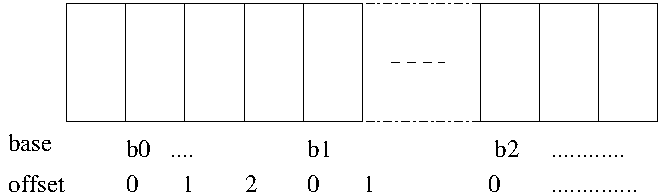
\includegraphics[height=4cm]{mem}
\end{center}
\caption{The {\it memory}}
\label{fig:mem}
\end{figure}


\subsection{Addresses}\label{ssec-store-addr}

The constructor for addresses is: 
\begin{description}
  \item{\whyinline{addr(b,ofs)}} returns an integer (which represent
an address). This integer is computed from a base
    \whyinline{b} and an offset \whyinline{ofs} (think about a binary
    applicative constructor)
\end{description} 

Two projections can be defined for such addresses: 
\begin{description}
  \item{\whyinline{base(x)}} returns the base of an address
    \whyinline{x} such that:\\  
    \whyinline{axiom base_addr: forall b,ofs:int. base(addr(b,ofs)) = b}
  \item{\whyinline{offset(x)}} returns the offset of an address
    \whyinline{x} such that:\\ 
    \whyinline{axiom offset_addr: forall b,ofs:int. offset(addr(b,ofs)) = ofs}
\end{description} 

An address can be shifted: 
\begin{description}
  \item \whyinline{addr_shift(a,ofs)} returns an address shifted of \whyinline{ofs} 
cells from the address \whyinline{a} such that \\ 
\whyinline{base (addr_shift(a,ofs)) = base(a)} and \\
\whyinline{offset (addr_shift(a,ofs)) = offset(a)+ofs}.
\end{description} 

An address \whyinline{a} has to be converted into a logic pointer
(see section~\ref{ssec-acsl-ptr}):\whyinline{pointer_of_addr(a)} and a logic
pointer \whyinline{p} can, also, be converted into an address:
\whyinline{addr_of_pointer(p)}.


\subsection{Blocks and zones}\label{ssec-store-addrg}

An address is too weak to specify the place into the heap where a
value is stored.  

\begin{figure}[ht!]
\begin{center}
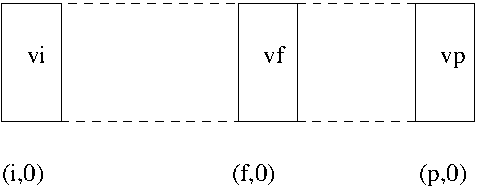
\includegraphics[height=4cm]{size_base}
\end{center}
\caption{Typed representation of objects}
\label{fig:sz_base}
\end{figure}

The address of base specifies the first cell where the value is stored, 
and a value is stored over a number of cells corresponding to the size of
this value (Think about some kind of C \whyinline{sizeof}, but more abstract.).
In the Store model, the size of values of basic types is $1$, 
this is the case of the integer \whyinline{i}, 
the float \whyinline{f} and the pointer \whyinline{p} in the 
figure~\ref{fig:sz_base}.
The size of a more complex value, such as an array and a record, is the 
number of objects of which it is comprised.
The figure~\ref{fig:sz_compl} considers the following code: 

\begin{ccode}
 struct S 
 { int f[2]; 
   float g;
 } ; 

 S s;
 
 S t[2];
\end{ccode}

\begin{figure}[ht!]
\begin{center}
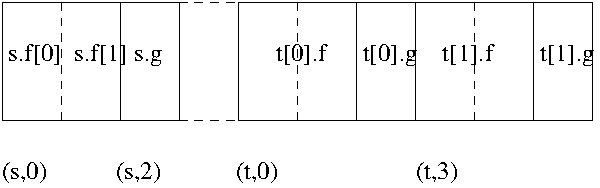
\includegraphics[height=4cm]{size_compl}
\end{center}
\caption{Typed representation of objects}
\label{fig:sz_compl}
\end{figure}



The representation of \whyinline{s} needs three cells in the {\it memory}, 
the representation of \whyinline{t} needs six cells, three for each 
element. 

\subsubsection{Blocks}\label{ssec-store-bloc}

The pair of an address and a
number of cells forms a block of {\it memory}.
The constructors of such bocks are:
\begin{description}
   \item{\whyinline{zempty}} is the empty block. Nothing can be stored 
     there. 
   \item{\whyinline{zrange(b,ofs,n)}} represents the {\it memory} block
     composed of the
     \whyinline{n} cells starting from the address \whyinline{addr(b,ofs)}. 
     This block can be used to load and store records and arrays in the 
     {\it memory}.
   \item \whyinline{zrange_of_addr(a)} returns the {\it memory} block
     composed of one cell for a basic type at the address \whyinline{a}.
     Its definition is: \\
     \whyinline{zrange_of_addr(a) = zrange(base(a),offset(a),1)}.
   \item \whyinline{zrange_of_addr_range(a,ofs,n)} returns the {\it memory}
     block of \whyinline{n} cells from the address \whyinline{a}
     shifted by \whyinline{ofs}.
     Its definition is: \\
     \whyinline{zrange_of_addr_range(a,ofs,n) = zrange(base(a),offset(a)+ofs,n)}.
\end{description}


Then, the validity of an address and the separation between two
addresses hang on the number of cells associated to the addresses:
\begin{description}
 \item{\whyinline{valid(ta,a,n)}} holds iff all \whyinline{n} cells
   from the address \whyinline{a} are included into the number of
   cells associated to the \whyinline{base(a)} into the allocation
   table \whyinline{ta}.
 \item{\whyinline{separated_on_addr(a,n,a',n')}} holds iff there is no
   overlap between the \whyinline{n} cells from \whyinline{a} and the
   \whyinline{n'} cells from \whyinline{a'}.
\end{description}


\subsubsection{Zones}\label{ssec-store-zone}

 The type \whyinline{zone} is defined as sets of 
 blocks. Blocks identify a number of adjacent cells related to an
 address of base, and zones allow the identification of any partition
 of the whole {\it memory}\/. \par

 In the logic language $\cal{L}$, block constructs are promoted to 
 singletons of type \whyinline{zone}.
 Just an union operator is necessary to build complex zones from zones
 and/or blocks. Zones can be compared using classical set operators:
 \begin{description}
   \item{\whyinline{zunion(z,z')}} unions of two {\it memory} zones.
   \item{\whyinline{included(z,z')}} holds if the {\it memory} zone
     \whyinline{z} is included in the {\it memory} zone \whyinline{z'}.
   \item{\whyinline{separated(z,z')}} holds if the {\it memory} zone \whyinline{z} does not
     intersect the {\it memory} zone \whyinline{z'}. This operation is used for
     the translation of \whyinline{\\separated} function of \textsf{ACSL}.
 \end{description}

 A zone equivalents to singleton is a particular zone since it defined a block which
 can content as well as basic data than complex data as arrays and records of $\cal{L}$.
 It is possible to recognize such zone: 
\begin{description}
   \item{\whyinline{is_bloc(z)}} holds if and only if it exists
   \whyinline{x, ofs>0, n>0} such that \whyinline{z = zrange(base(x),ofs,n)}.
\end{description}
 

 The validity of a location, the \textsf{ACSL} predicate
 \cinline{valid(l)} is translated as \whyinline{valid(ta,addr_of(l),n)} when
 \whyinline{n} is the number of cells of the location \whyinline{l}.

 The separation of two location, the \textsf{ACSL} predicate
 \cinline{separated(l,l')} is translated by 
 \whyinline{separated(zone_of(l),zone_of(l'))}


\subsection{Variable scope}

The allocation table informs about how many cells have
been allocated for each address of base. 
As said in section~\ref{ssec-store-addrg}, querying the
allocation table defines the validity of an address for a number of
cells. It can also informs about the scope of variables.  An unallocated
\whyinline{base(x)} is associated to $0$ cell into the allocation
table. \par

Moreover, we need a property over \whyinline{base(x)} parametrized
by a store and a allocation to hang on the bound of the C variable $x$
scope. Hence, the property \whyinline{is_fresh(m,ta,b)} means that all
addresses such as their base is \whyinline{b}, cannot be loaded into the
store \whyinline{m} and cannot be valid into \whyinline{ta}. \par


During a WP computation, the scope of different kinds of variables 
is specified as follows:
\begin{description}
  \item Global variables are marked as they are already allocated into 
the initial allocation table, 
 \item Formal parameters are specified as they were out of the scope
   of the initial memory configuration. Their scopes are open before
   the precondition,
  \item The local variables scopes are open after the precondition and are
  closed before the post-condition.
\end{description}

Lets consider the following piece of code:
\begin{ccode}

int X;

/*@ requires \valid(p);
    assigns *p;
    ensures  *p == X;
*/
void f (int *p)
{
 int * q; 
 q=p;
 *q = X;

}

\end{ccode}


 Running the WP computation with the Store model we get the 
following environment : 
\begin{whycode}
Global 'X'
wp_store_ex.c:1: int X ;
function X_X () : int = 2

Local 'p'
wp_store_ex.c:7: int* p ;
function X_p () : int = 1

Local 'q'
wp_store_ex.c:9: int* q ;
function X_q () : int = 3

Global 'X'
wp_store_ex.c:1: Global allocation table
axiom Alloc_X: forall ta:int farray.
     global(ta)
  -> (ta[X_X] = 1)
\end{whycode}

 For each C variable, a base is defined \whyinline{X_X,X_p,X_q}.  The
 axiom \whyinline{Alloc_x} specifies the global scope of the variable
 \whyinline{X}. If we get the scope mark \whyinline{global(ta)} then 
 \whyinline{X} is valid in \whyinline{ta} and the size associated is 
 \whyinline{1}.  
  

 The WP computation for the post-condition produces the formula:

 \begin{whycode}
 forall m_0:data farray.
  forall ta_0:int farray.
     global(ta_0) 
  -> (ta_0[X_p] = 0)
  -> is_fresh(m_0, ta_0, X_p)
  -> (let ta_0= ta_0[X_p->1] in
         valid(ta_0, {m_0[addr(X_p,0)]}, 1)
      -> (ta_0[X_q] = 0)
      -> is_fresh(m_0, ta_0, X_q)
      -> (let ta_0= ta_0[X_q->1] in
          let m_1= m_0[addr(X_q,0)->{{m_0[addr(X_p,0)]}}] in
          let m_2= m_1[{m_1[addr(X_q,0)]}->{{m_1[addr(X_X,0)]}}] in
          let ta_0= ta_0[X_q->0] in
             is_fresh(m_2, ta_0, X_q)
          -> (let ta_0= ta_0[X_p->0] in
                 is_fresh(m_2, ta_0, X_p)
              -> ({m_2[{m_0[addr(X_p,0)]}]} = {m_2[addr(X_X,0)]})))) 
 \end{whycode}

First, the {\it memory} and the allocation table are introduced. 
The first hypothesis, \whyinline{global(ta_0)},
triggers the axiom \whyinline{Alloc_X} and we have \whyinline{X}
already allocated in the initial allocation table. 

The two next hypotheses: 
  \begin{whycode}
 (ta_0[X_p] = 0)
  -> is_fresh(m_0, ta_0, X_p) 
 \end{whycode}

say that the formal parameter \whyinline{p} is out of the scope of the
initial memory configuration: its base of address is not valid in the 
allocation table and it cannot been loaded in the initial memory.

As formal parameters are in the scope of the precondition, 
the allocation table has to be updated before the precondition computation.
After the precondition translation, the two hypotheses
 
\begin{whycode}
  (ta_0[X_q] = 0)
  -> is_fresh(m_0, ta_0, X_q)
\end{whycode}
 
state that the local variable \whyinline{q} is out of the scope of
the precondition and then the allocation table is updated before
formulating the body of the function.
Before asserting the post-condition, the scope of the local variable 
is closed: the allocation table is updated and its address cannot be 
loaded in the final memory. On the contrary, the scope of the formal
parameter is still open, since the formal parameters are in the scope 
of the post-condition. 

\subsection{The store operations}
  
 The store is an array of \whyinline{data} indexed by addresses
 (see figure~\ref{fig:mem} and section~\ref{ssec-acsl-rec} 
 for the logic records).


\subsubsection{Data}\label{ssec-acsl-value}

 The store is specified into logic array of
 \whyinline{data}, indexed by addresses. The type \whyinline{data} is a
 common type representation for all types of values supported by the
 \textsf{ACSL}. That means a field of type $\tau$ contains an object
 of type \whyinline{data} in the representation of the
 record. However, the value of a field of type $\tau$ must be
 specified by an object of type $\tau$. 




 \subsubsection{Loading and assignment of basic objects}
   As basic type object only needs one cell to be stored in the Store
   model, loading/writing a value of a basic type are translated in
   simple access/update from the store, but this value has to be
   encoded/decoded as defined in section~\ref{ssec-acsl-rec}. The format
   for integers and floats are thus defined in section~\ref{ssec-acsl-rec},
   for store address, we specify the special format
   \whyinline{addr_format}.
   
   
 \subsubsection{Loading and assignment of records and arrays}
 
   In the Store model, it is possible to load or assign records or
   arrays using the combination of two steps. 

   First, loading and assignment of a block of \whyinline{data} in
   the memory:
   \begin{description}
    \item{\whyinline{access_range(m,z)}} loads in one time a zone
       \whyinline{z} in the memory \whyinline{m} and returns a
      \whyinline{data}. Note that \whyinline{z} has to be 
      \whyinline{zrange(b,ofs,n)} with \whyinline{n >0} to make sense. 
      This is what ensured the predicate \whyinline{is_block(z)}.
      
      \item{\whyinline{update_range(m,z,v)}} updates in one operation
        the zone \whyinline{z} by the \whyinline{data} \whyinline{v}
        in the memory \whyinline{m}, with \whyinline{is_block(z)}.
   \end{description}

   Secondly, decoding/encoding the data (involved in the first step)
   with the format of the type of the object. 

   The two following example illustrate this mechanism.

   Suppose this simple function:

   \begin{ccode}
   int t[4]; 
   /*@ assigns t[1]; 
    ensures t == {\old(t) \with [1] = (int)3}; 
   */

  void modif_array(void)
  { t[1] =3;}

   \end{ccode}

  
   The generated output in $\cal{L}$ defines, at first, how to update
   and access to indexed values of the array of $4$ int: 

   \begin{whycode}

axiom Loaded_int_4_idx:
  forall m:data farray.
  forall p:int.
  forall i:int.
     (0 <= i)
  -> (i < 4)
  -> (decode(Afmt_int_4,access_range(m,zrange_of_addr_range(p,0,4)))[i]
      = decode(int_format,m[addr_shift(p,i)]))
axiom Updated_int_4:
 forall m:data farray.
 forall i:int.
 forall e:int.
 forall p:int.
    (0 <= i)
 -> (i < 4)
 -> Eqarr_int_4(
     decode(Afmt_int_4,
        access_range(m[addr_shift(p,i)<-encode(int_format,e)],
          zrange_of_addr_range(p,0,4))),
     decode(Afmt_int_4,access_range(m,zrange_of_addr_range(p,0,4)))[i<-e])
 \end{whycode}
   

Notice that the update definition requires the equality of array of
$4$ int (definition \whyinline{Eqarr_int_4}) defined in the
\textsf{ACSL} model see section~\ref{ssec-acsl-eq}. \par 


In the Store model, the access to the whole array \whyinline{t} is the
 \whyinline{data} loaded from a block of the store \whyinline{m},
 starting from the address \whyinline{(p,0)} over $4$ cells :
\whyinline {access_range(m,zrange_of_addr_range(p,0,4))}. This
\whyinline{data} is decoded as an array of $4$ int. The axiom
\whyinline{Loaded_int_4_idx} expresses that accessing to the $i^{nth}$
index of this array is the same that accessing to the address of the
beginning of the array \whyinline{p} shifted by $i$ times the size of
\whyinline{int} (i.e. $1$ since int is a basic type).
The update operation is defined in the same flavor. \par 


The postcondition is formulated as: 
\begin{whycode}
goal store_full_modif_array_post_1:
  forall m:data farray.
  Eqarr_int_4(
    decode(Afmt_int_4,
      access_range(m[addr(X_t,1)<-encode(int_format,3)],zrange(X_t,0,4))),
    decode(Afmt_int_4,access_range(m,zrange(X_t,0,4)))[1
      <-as_int(sint32_format,3)])
\end{whycode}
 Informally, it is to say that the array \whyinline{t} loaded in the memory
 after having updated the cell at the address \whyinline{addr(X_t,1)}
 with the \whyinline{data} encoding of the int \whyinline{3} is equal
 to the updated array loaded in the memory
 \whyinline{decode(Afmt_int_4,access_range(m,zrange(X_t,0,4)))} at
 index \whyinline{1} with the \whyinline{data} encoding of the int
 \whyinline{3}.\par

 \whyinline{Afmt_int_4} is the format of array of $4$ int for the Store
  model. The model Store generated its own format for each array
  and record type. \par



 In the case of a record, the same kind of definitions occurs but this
 time, instead of generalize over all bound indexed (\whyinline{0 <= i} 
 and \whyinline{i < 4}) an axiom for loading and another for
 storing are defined for each field of the record. \par

  
\subsection{The assigns clause specification}

  The WP computation needs two different specifications of an assigns
  clause:
\subsubsection{Assigns as a memory operation} 
 The memory operation \whyinline{update_havoc(m,z,v)} returns a memory
 where all addresses contains in the zone \whyinline{z} contains a
 \whyinline{data}.  This function is quite similar than
 \whyinline{update_range} at first glance. In fact, they are
 different, \whyinline{z} can be any zone and the stored
 \whyinline{x} is never encoded or decoded.

\subsubsection{Assigns as a property between two memory states}

 In the Store model there are two different ways to express the assigns clause
 as a goal: 
 \begin{description}
    \item{Relational:} the predicate
      \whyinline{is_havoc(ta_init,m_init,z,ta_fin,m_fin)} holds if
      from the memory configuration \whyinline{(ta_init,m_init)} to
      \whyinline{(ta_fin,m_fin)} excluded all addresses in the zone
      \whyinline{z} nothing has changed.
      
%    \item{Zone inclusions:} TODO Lo�c... \whyinline{included(z_c,z_a)}
 \end{description}
 



%% %% Chapter WP Models

\section{Runtime}\label{sec-runtime}

\subsection{Description and limitations}

This model is a very low level one, where the memory is just a big array of bits
indexed by addresses. The values, represented by bit vectors 
(\whyinline{bits}),
are stored in memory zones (\whyinline{rt_zone})
represented by a starting address, and a size (number of bits).
The  \whyinline{rt_load(m, z)} operation returns the bits stored in the zone
\whyinline{z}
of the memory \whyinline{m}, and \whyinline{rt_store (m, a, b)} returns a memory similar to
\whyinline{m} except that the bits \whyinline{b} have been stored at the address
\whyinline{a}.

Operations \whyinline{rt_to_bits} and \whyinline{rt_from_bits} specify
how to interpret the bit vectors into typed values.
In simple cases, we don't need to go into representation details,
but it can be necessary when the C program uses some casts
and other architecture dependent features
such as endianness for instance.

This model also deals with memory management of variables 
(see \whyinline{rt_valloc} and \whyinline{rt_vfree})
to be able to prove the validity of pointers,
but the dynamic allocations are not handled yet.

\subsection{Examples}

\subsubsection{Simple variable assignment}

Let's begin with the simple assignment example used in Hoare presentation.
To check this assertion after this statement:
\begin{ccode}
  x = y+1;
  //@ assert x > 0;
\end{ccode}
the proof obligation with the Runtime model is a lot more complex:
\begin{whycode}
  forall ma:memalloc.
  forall mb:memory.
  let mb=
    rt_store(mb,rt_vaddr(ma,X_x),
      rt_to_bits(sint32_format,
        (rt_from_bits(rt_load(mb,rt_vzone(ma,X_y)),sint32_format)+1))) in
  (0 < rt_from_bits(rt_load(mb,rt_vzone(ma,X_x)),sint32_format))
\end{whycode}
First of all, we see that the memory state is represented by two variables:
$ma$ is used for allocation information, and $mb$ for the values (bits).
The last line is the translated initial property which say that if we read
(\whyinline{
rt_load}) in $mb$ the bits stored in the zone where $x$ is allocated
(\whyinline{
rt_vzone(ma,X_x)}), and if we interpret (\whyinline{rt_from_bits})
those bits as a signed 32 bit integer (which is the type of $x$),
then we should get a positive value.
The other lines represent the bit memory update (\whyinline{rt_store(mb,...)})
due to the assignment.

Trying to complete the proof, the Runtime model requires us to prove
that \cinline{(y+1)} still fits in the \whyinline{sint32_format} which hasn't
been requested by the Hoare model because of its abstraction level.
This condition is implied by the RTE generated annotations
that should be check separately (see \verb!-rte! option).

This example might look a little frightening because of the size of the proof
obligation compared to the size of the code, and that is precisely why 
it is not advisable to use the Runtime model when its low level features are not
required. But we will see in \S\ref{sec-funvar} that in some simple cases,
such as this one, dramatic simplifications can be done.


\subsubsection{Simple variable allocation}

Runtime model defines the operation \whyinline{rt_valloc} to represent
a modification of the allocation information. So checking the assertion
\begin{ccode}
  int x;
  //@ assert \valid (&x);
\end{ccode}
gives the following the proof obligation:
\begin{whycode}
  forall ma:memalloc.
  let ma= rt_valloc(ma,X_x,32) in
  rt_valid(ma, rt_vzone(ma,X_x))
\end{whycode}
which is trivially true according to Runtime properties.

Conversely, the operation \whyinline{rt_vfree} is used to represent
the deallocation. It makes possible to check this kind of property:
\begin{ccode}
  { int x; p = &x; }
  //@ assert ! \valid (p);
  \end{ccode}
That gives the following proof obligation:
\begin{whycode}
  forall ma:memalloc.
  forall mb:memory.
  let ma1 = rt_valloc(ma,X_x,32) in
  let mb= rt_store(mb,rt_vaddr(ma1,X_p),
             rt_to_bits(rt_addr_format,rt_vaddr(ma1,X_x_0_1))) in
  let ma2= rt_vfree(ma1,X_x_0_1) in
  (not rt_valid(ma2,
      rt_zone(rt_from_bits(rt_load(mb,rt_vzone(ma2,X_p)),rt_addr_format),32)))
\end{whycode}
but could be simplified, using Runtime rules, to:
\begin{whycode}
  forall ma:memalloc.
  let ma1 = rt_valloc(ma0,X_x,32) in
  let ma2= rt_vfree(ma1,X_x) in
  not rt_valid (ma2, rt_zone(rt_vaddr(ma1,X_x), 32))
\end{whycode}
which is true because, of course, a zone is not valid after having been freed.

%% \section{Logic variables}\label{sec-funvar}

As previously presented, there is two kinds of memory models.  One
based on variables, as in the Hoare model see section~\ref{sec-hoare}
and the other based on the representation of the heap, as the Store
model (see section~\ref{sec-store}) and the Runtime model (see
section~\ref{sec-runtime}).

The second kind of memory model is more expressive since it can handle
 dereferencing of pointers, and addresses of variables. 
The cost is quite heavy: the generated formula are largest.

The ideal is to benefit this expressiveness only for the variables
involved in dereferencing of pointers and address management, in
other words the variables such as their addresses are computed. For
the other variables, variables such as their addresses are never
computed (notice that they behave as functional or logical variables)
they can be handled by a model {\it � la} Hoare. This kind of
optimization, with a generous definition of optimization, is quite
current in memory model specifications and implementations.

In the WP, the model {\it � la} Hoare is the Logicvar model and
to make it cooperate with a based on heap memory model, one has to set
the {\tt -wp-logicvar}.

A variable translated in Logicvar has in $\cal{L}$ a logic type then
it is translated as \textsf{ACSL} data (see section~\ref{sec-acsl}).


Let us consider this example: 
\begin{ccode}
typedef struct S { int a; int * p; }; 

struct S s;
struct S r;


/*@ 
    ensures \result == {s \with .a = (int)4 };
*/
struct S ret_struct(void)
{
  struct S * ps; 
  r.a = s.a ; 
  s.a = 4;
  ps = &r;
  return r;
}
\end{ccode}

This example has a semantics only in a based on heap memory model,
because the address of \whyinline{r} is taken. Computing the 
proof obligation associated to the post-condition with the memory model 
Store in the WP plug-in gives:

\begin{whycode}

goal store_full_ret_struct_post_1:
  forall m:data farray.
  forall ta:int farray.
     global(ta)
  -> (ta[X_ps] = 0)
  -> is_fresh(m, ta, X_ps)
  -> is_fresh(
       m[addr(X_r,0)
         <-encode(int_format,decode(int_format,m[addr(X_s,0)]))][addr(X_s,
                                                                    0)
         <-encode(int_format,4)][addr(X_ps,0)
         <-encode(addr_format,addr(X_r,0))], ta_2[X_ps<-1][X_ps<-0], X_ps)
  -> Eqrec_S(
       decode(Cfmt_S,
         access_range(
           m[addr(X_r,0)
             <-encode(int_format,decode(int_format,m[addr(X_s,0)]))][
             addr(X_s,0)
             <-encode(int_format,4)][addr(X_ps,0)
             <-encode(addr_format,addr(X_r,0))],zrange(X_r,0,2))),
       decode(Cfmt_S,
         access_range(
           m[addr(X_r,0)
             <-encode(int_format,decode(int_format,m[addr(X_s,0)]))][
             addr(X_s,0)
             <-encode(int_format,4)][addr(X_ps,0)
             <-encode(addr_format,addr(X_r,0))],zrange(X_s,0,2)))[F_a
         <-encode(int_format,as_int(sint32_format,4))])
\end{whycode}

For each variable, a location is created into the heap.  The local
variables trigger two local allocations for their locations.  The three
assignments take place in the same $\cal{L}$ array, the store.
Unless expressing the address taken of \whyinline{r} and the address
assignment \whyinline{ps= &r;}, this is uninteresting to use the Store
model. Moreover, this assignment is heavy noise for the automatic
provers. Then, using Logicvar, the WP plug-in generates the formula:

\begin{whycode}
goal store_ret_struct_post_1:
  forall m:data farray.
  forall s:data farray.
  Eqrec_S(
    decode(Cfmt_S,
      access_range(
        m[addr(X_r,0)<-encode(int_format,decode(int_format,s[F_a]))],
        zrange(X_r,0,2))),
    s[F_a<-encode(int_format,4)][F_a
      <-encode(int_format,as_int(sint32_format,4))])
\end{whycode}

Since the assignment \whyinline{ps= &r;} is {\it mute} for the post-condition, 
the WP plug-in ignores it. Hence, only \whyinline{r} is represented into the 
memory, the other variables are handled as logic variables.




% vim: spell spelllang=en

